\subsection{\textit{Large-Scale Provisioning of
    Resource Constrained
    IoT Deployments, LEONORE}}
\label{subsec:leonore}

Riset dilakukan oleh Michael Vogler, Johannes M. Schleicher, Christian Inzinger, Stefan Nastic, Sanjin Sehic and Schahram Dustdar dari Vienna University of Technology. Riset ini menjelaskan mengenai cara pembuatan sebuah infrastruktur untuk melakukan \textit{provisioning} perangkat \textit{IoT} dalam skala besar. Penelitian ini berfokus untuk membuat sebuah pendekatan terstruktur dalam menyediakan layanan deployment lingkungan IoT dengan dua metode yaitu Push dan Pull.

LEONORE dibuat untuk menyelesaikan tantangan yaitu mengelola jutaan perangkat \textit{IoT} yang heterogen pada sistem skala besar yang memiliki pada domain \textit{smart city}. Solusi yang sudah ada sering kali, bersifat \textit{partial} ataupun manual dalam menangani sebagian infrastruktur. Tentunya, Hal ini tidak efisien dan mahal karena membutuhkan banyak tenaga kerja. Oleh karena itu, LEONORE menghadirkan solusi provisioning yang skalabel dan elastis untuk mengelola perubahan dan kebutuhan baru.

Arsitektur LEONORE dibuat dengan membuat 4 API yang dapat diakses oleh mulai dari  \textit{User API, Repository API, Device API, serta Provisioning}. Arsitektur ini memilki cara kerja yaitu menyimpan seluruh image atau dapat disebut sebagai deployment plan pada \textit{repository}, apabila repository membutuhkan dependency lain maka akan diletakan pada bagian \textit{artifact}. Artifact dibuat dan di proses oleh \textit{package builder} yang seluruh \textit{resources} nya diatur oleh komponen manajemen yaitu \textit{package, dependency management serta gateway management}. Setelah siap untuk di\textit{deploy}, bagian \textit{iot gateway handler} melakukan provisioning kepada target \textit{device}. Secara umum arsitektur leonore dapat dilihat pada gambar \ref{fig:arsitektur-leonore}

\begin{figure}[ht]
  \centering
  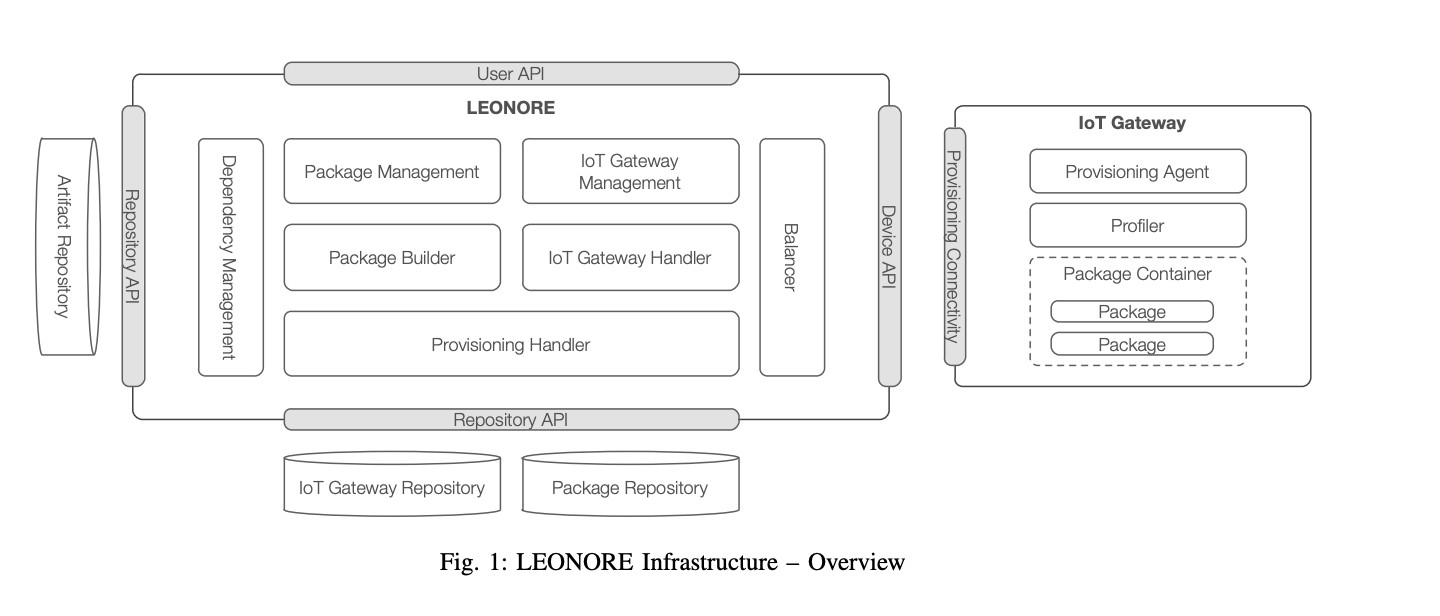
\includegraphics[width=0.8\textwidth]{resources/chapter-2/arsitektur-leonore.jpg}
  \caption{Arsitektur Leonore \parencite{vogler2015leonore}}
  \label{fig:arsitektur-leonore}
\end{figure}

Illustrasi cara kerja LEONORE dapat dilihat pada gambar \ref{fig:sequence-leonore}. Berikut adalah cara kerja dari sistem LEONORE:
\begin{enumerate}
  \item Mengecek Ketersediaan \textit{Artifact}.
  \item Mengambil \textit{Iot Gateway} sebagai group yang akan di \textit{deploy}.
  \item \textit{Delegate deployment} task ke setiap \textit{IoT Gateway}.
  \item Analisa kompatibilitas untuk setiap nodes.
  \item Resolve \textit{dependency} dan membuat \textit{application package} sesuai dengan group \textit{IoT Gateway}
  \item Jalankan \textit{provisioning}
  \item Tunggu hingga setiap nodes selesai lalu lakukan cek untuk setiap nodes hingga proses selesai
\end{enumerate}

\begin{figure}[ht]
  \centering
  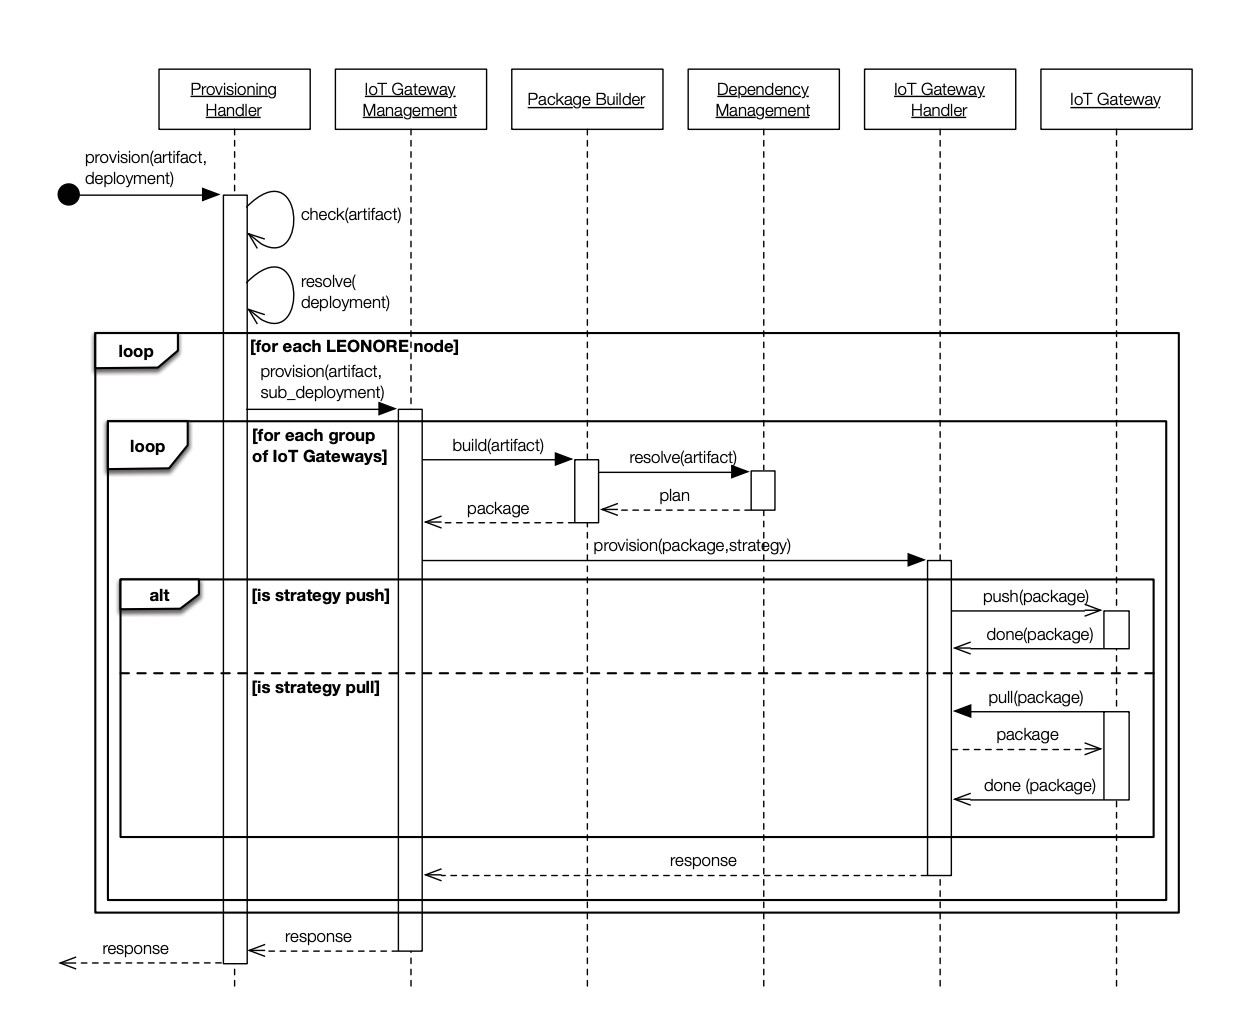
\includegraphics[width=0.8\textwidth]{resources/chapter-2/leonore-sequence.jpg}
  \caption{Sequence Diagram Proses \textit{Deployment} LEONORE \parencite{vogler2015leonore}}
  \label{fig:sequence-leonore}
\end{figure}

Untuk mengevaluasi kinerja LEONORE, dilakukan pengujian pada \textit{cloud}, berisi 1000 perangkat yang divirtualisasi menggunakan \textit{docker}. Hasilnya LEONORE dapat melakukan \textit{provisioning} seluruh perangkat dengan waktu yang \textit{reasonable}. Metode \textit{pull provisioning} menghasilkan latensi yang tinggi dibandingkan metode \textit{push} yang memberikan hasil yang cukup baik.